\documentclass[aps,prb,onecolumn,groupedaddress,notitlepage,showpacs,floatfix,superscriptaddress]{revtex4-1}
\usepackage{times,amsmath,amsfonts,amssymb,mathrsfs,graphics,graphicx,color,comment,bm}
\usepackage[dvips]{epsfig}
\usepackage[pdfstartview=FitH]{hyperref}
\usepackage{natbib}
\usepackage{appendix}
\usepackage{epstopdf}
\usepackage[export]{adjustbox}
\hypersetup{
colorlinks=true,       	
linkcolor=blue,          	
citecolor=blue,        
filecolor=blue,      	
urlcolor=blue,           	
runcolor=blue
}
\newcommand{\ignore}[1]{}
%%%%%%%%%%%%%%%%%%%%%%%%%%%%%%%%%%%%%%%%%%%%%%%%%%%%%%%%%%%%%%%%
\let\oldsqrt\sqrt
\def\sqrt{\mathpalette\DHLhksqrt}
\def\DHLhksqrt#1#2{%
\setbox0=\hbox{$#1\oldsqrt{#2\,}$}\dimen0=\ht0
\advance\dimen0-0.2\ht0
\setbox2=\hbox{\vrule height\ht0 depth -\dimen0}%
{\box0\lower0.4pt\box2}}

%%%%%%%%%%%%%%%%%%%%%%%%%%%%%%%%%%%%%%%%%%%%%%%%%%%%%%%%%%%%%%%%
% in: s * [x], "x" is the magnification factor
\DeclareFontFamily{OT1}{pzc}{}
\DeclareFontShape{OT1}{pzc}{m}{it}%
              {<-> s * [1.25] pzcmi7t}{}
\DeclareMathAlphabet{\mathpzc}{OT1}{pzc}%
                                 {m}{it}
%%%%%%%%%%%%%%%%%%%%%%%%%%%%%%%%%%%%%%%%%%%%%%%%%%%%%%%%%%%%%%%%
%%%%%%%%%%%%%%%%%%%%%%%%%%%%%%%%%%%%%%%%%%%%%%%%%%%%%%%%%%%%%%%%

\begin{document}
\title{Time evolution by the means of unitary MERA-like tensor network operator}
\author{R. Haghshenas}
%\affiliation{Department of Physics, Sharif University of Technology, P. O. Box
%11155-9161, Tehran, Iran}
%\email{haghshenas@physics.sharif.edu}
%\date{\today}
%\begin{abstract}
%\end{abstract}
\maketitle

The optimized unitary $U$ obtained from e.g. MPO-optimization diagonalizes the Hamiltonian H
\begin{equation*}
U^{\dagger}HU=D=\sum_{\{ \tau  \}} E_{\{\tau\}}|\tau\rangle\langle \tau |=\sum_{\{ \tau  \}} E_{\{\tau\}}|\tau_{1}\cdots \tau_{N}\rangle\langle \tau_{1}\cdots \tau_{N} |, 
\end{equation*}
where $\{\tau\}$ forms a basis for Hilbert space, $E_{\{\tau\}}$ is energy spectrum and $D$ is a diagonal matrix, where value of energy is sitting  on diagonal elements. The following figure show the tensor network representation of unitary $U$.
\begin{center}
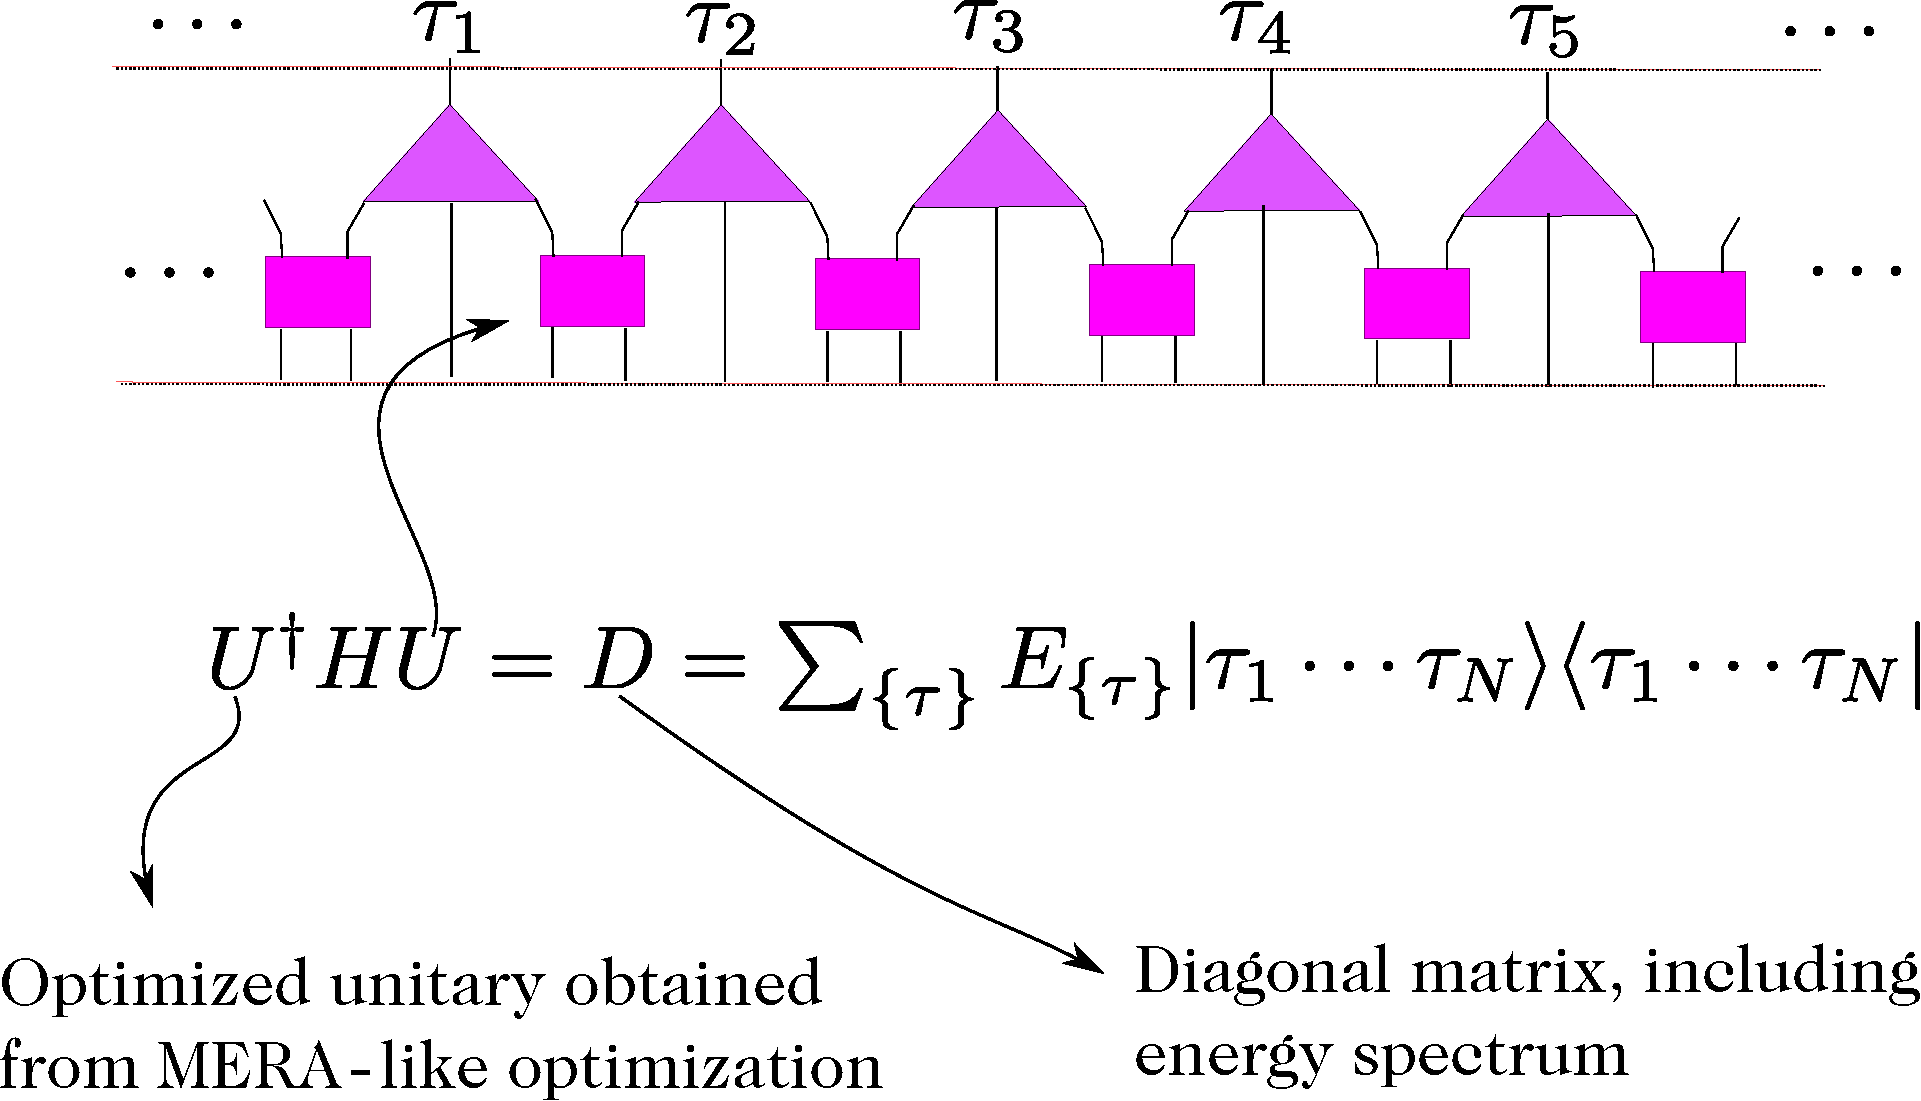
\includegraphics[scale=0.3, angle=0, origin=c]{Unitary-tensor-network}
\end{center}
Since MERA-like tensor network preserve locality of Hamiltonian, if you map the original Hamiltonian into upper layers of MERA, it still remains local in the sense that you could write it in terms of local operators. So, we could come to the following `key equation'
\begin{equation}
\text{key equation}\rightarrow E_{\{\tau\}}=\sum_{i}  O_{\tau_{i}, \tau_{i+1}}.
\label{EQ:keyEQ}
\end{equation}
Tensor network representation of operator $O_{\tau_{i}, \tau_{i+1}}$ has the following form,             
\begin{center}
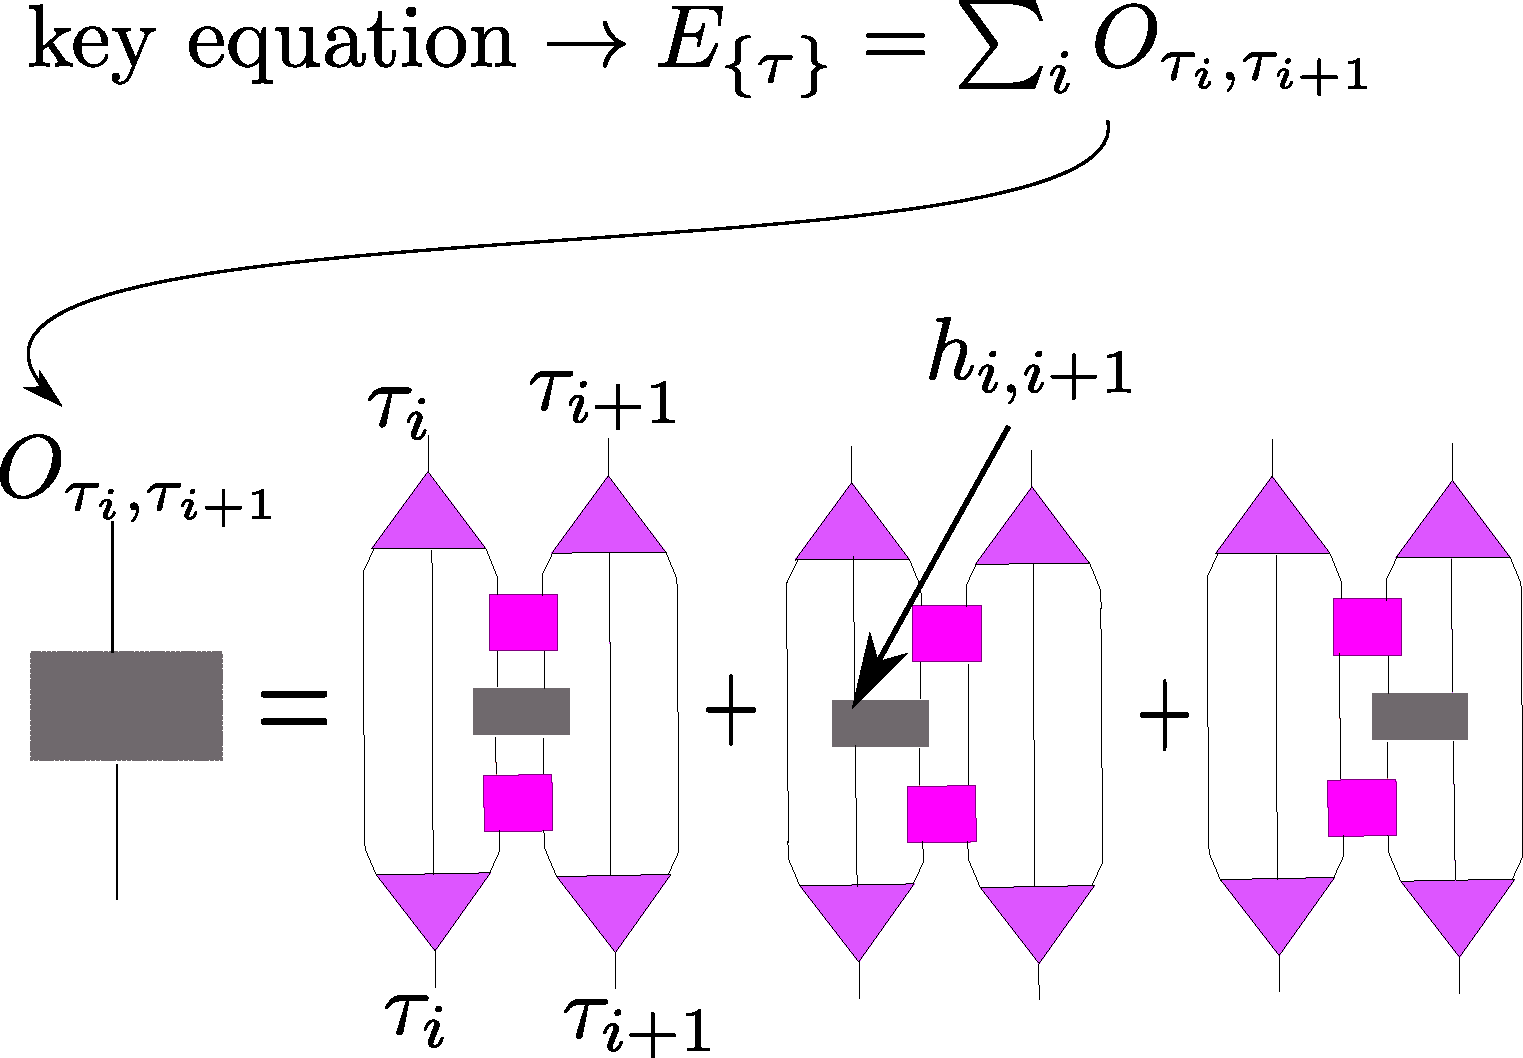
\includegraphics[scale=0.3, angle=0, origin=c]{Rg-MERA}
\end{center}
where terms $h_{i,i+1}$ are making the original Hamiltonian, $H=\sum_{i} h_{i,i+1}$. 


Our aim is to calculate time evolution of local quantity, such as below,
\begin{equation*}
\langle \psi(t) | \sigma^{z} |\psi(t)\rangle=\langle \psi(0)| U e^{iDt} U^{\dagger} \sigma^{z} U e^{-iDt} U^{\dagger}|\psi(0)\rangle.
\end{equation*}
The term $U^{\dagger} \sigma^{z} U$ finds a simple form as comes          
\begin{equation*}
U^{\dagger}\sigma^{z}  U   =\overline{\sigma} _{\tau'_{j},\tau_{j}}
\end{equation*}        
where index $j$ shows place of the $j$th particle, where $\sigma^{z}$ is acting. The tensor netwrork representation for above equation       
\begin{center}
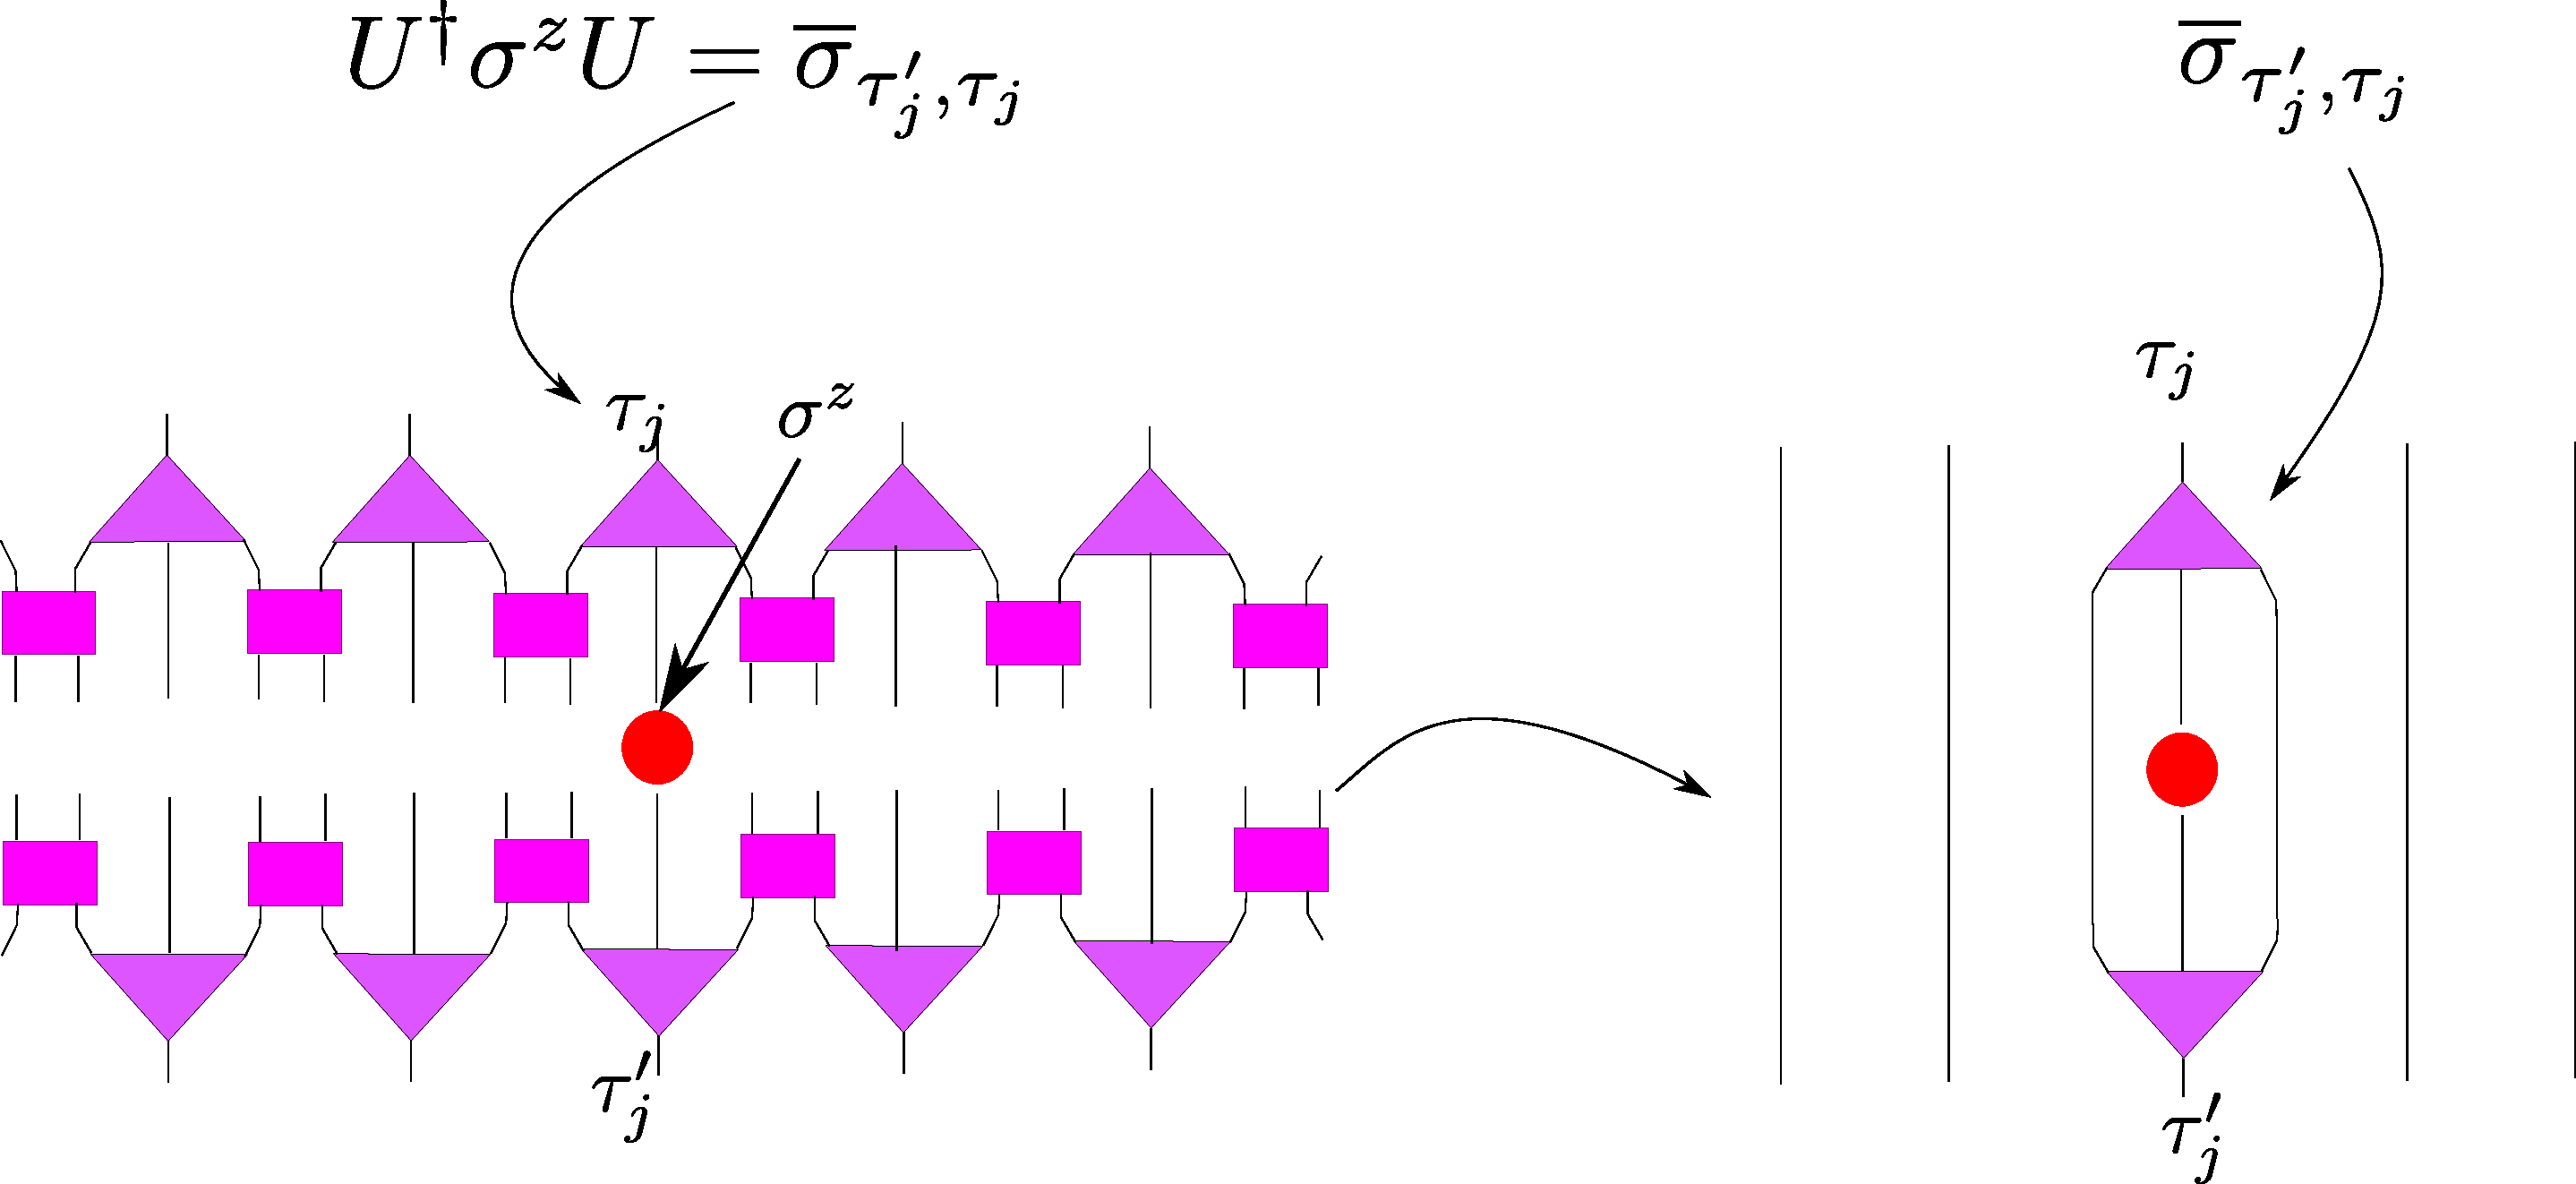
\includegraphics[scale=0.25, angle=0, origin=c]{unitary-local-operator}
\end{center}
has been drawn in above figure. By using this equation we could go further and write the following,

\begin{eqnarray*}
e^{iDt} U^{\dagger} \sigma^{z} U e^{-iDt}&=e^{iDt} \overline{\sigma} e^{-iDt}=\sum_{\{\tau,\tau'\}}  e^{-it(E_{\{\tau\}}-E_{\{\tau'\})} } \langle \tau'| \overline{\sigma}|\tau \rangle |\tau \rangle \langle\tau'|
\end{eqnarray*}
Since $ \langle \tau'| \overline{\sigma}|\tau\rangle=\delta_{\tau'_{1},\tau_{1}} \cdots \overline{\sigma} _{\tau'_{j},\tau_{j}}  \cdots  \delta_{\tau'_{N},\tau_{N}}$ and also by using key equation (Eq.~\ref{EQ:keyEQ}), we come to the following result,
\begin{equation*}
e^{iDt} U^{\dagger} \sigma^{z} U e^{-iDt}=I\otimes\cdots\otimes\mathcal{O}_{\tau'_{j-1}\tau'_{j}\tau'_{j+1};\tau_{j-1}\tau_{j}\tau_{j+1} } \otimes \cdots I
\end{equation*}
where operator $\mathcal{O}_{\tau'_{j-1}\tau'_{j}\tau'_{j+1};\tau_{j-1}\tau_{j}\tau_{j+1} }$ has the following form
\begin{equation*}
\mathcal{O}_{\tau'_{j-1}\tau'_{j}\tau'_{j+1};\tau_{j-1}\tau_{j}\tau_{j+1} }=\sum_{\tau'_{j-1}\tau'_{j}\tau'_{j+1};\tau_{j-1}\tau_{j}\tau_{j+1}} 
e^{-it(O_{\tau_{j-1},\tau_{j}}+O_{\tau_{j},\tau_{j+1}}-O_{\tau'_{j-1},\tau'_{j}}-O_{\tau'_{j},\tau'_{j+1}})}       
\overline{\sigma} _{\tau'_{j},\tau_{j}}    \delta_{\tau'_{j-1},\tau_{j-1}} \delta_{\tau'_{j+1},\tau_{j+1}}. 
\end{equation*}
Therefore, time evolution of local operator gets the simple form, 
\begin{equation*}
\langle \psi(t) | \sigma^{z} |\psi(t)\rangle=\langle \psi(0)|U\mathcal{O} U^{\dagger}|\psi(0)\rangle.
\end{equation*}
so that the graphical representation of above equation will take the below figure.
\begin{center}
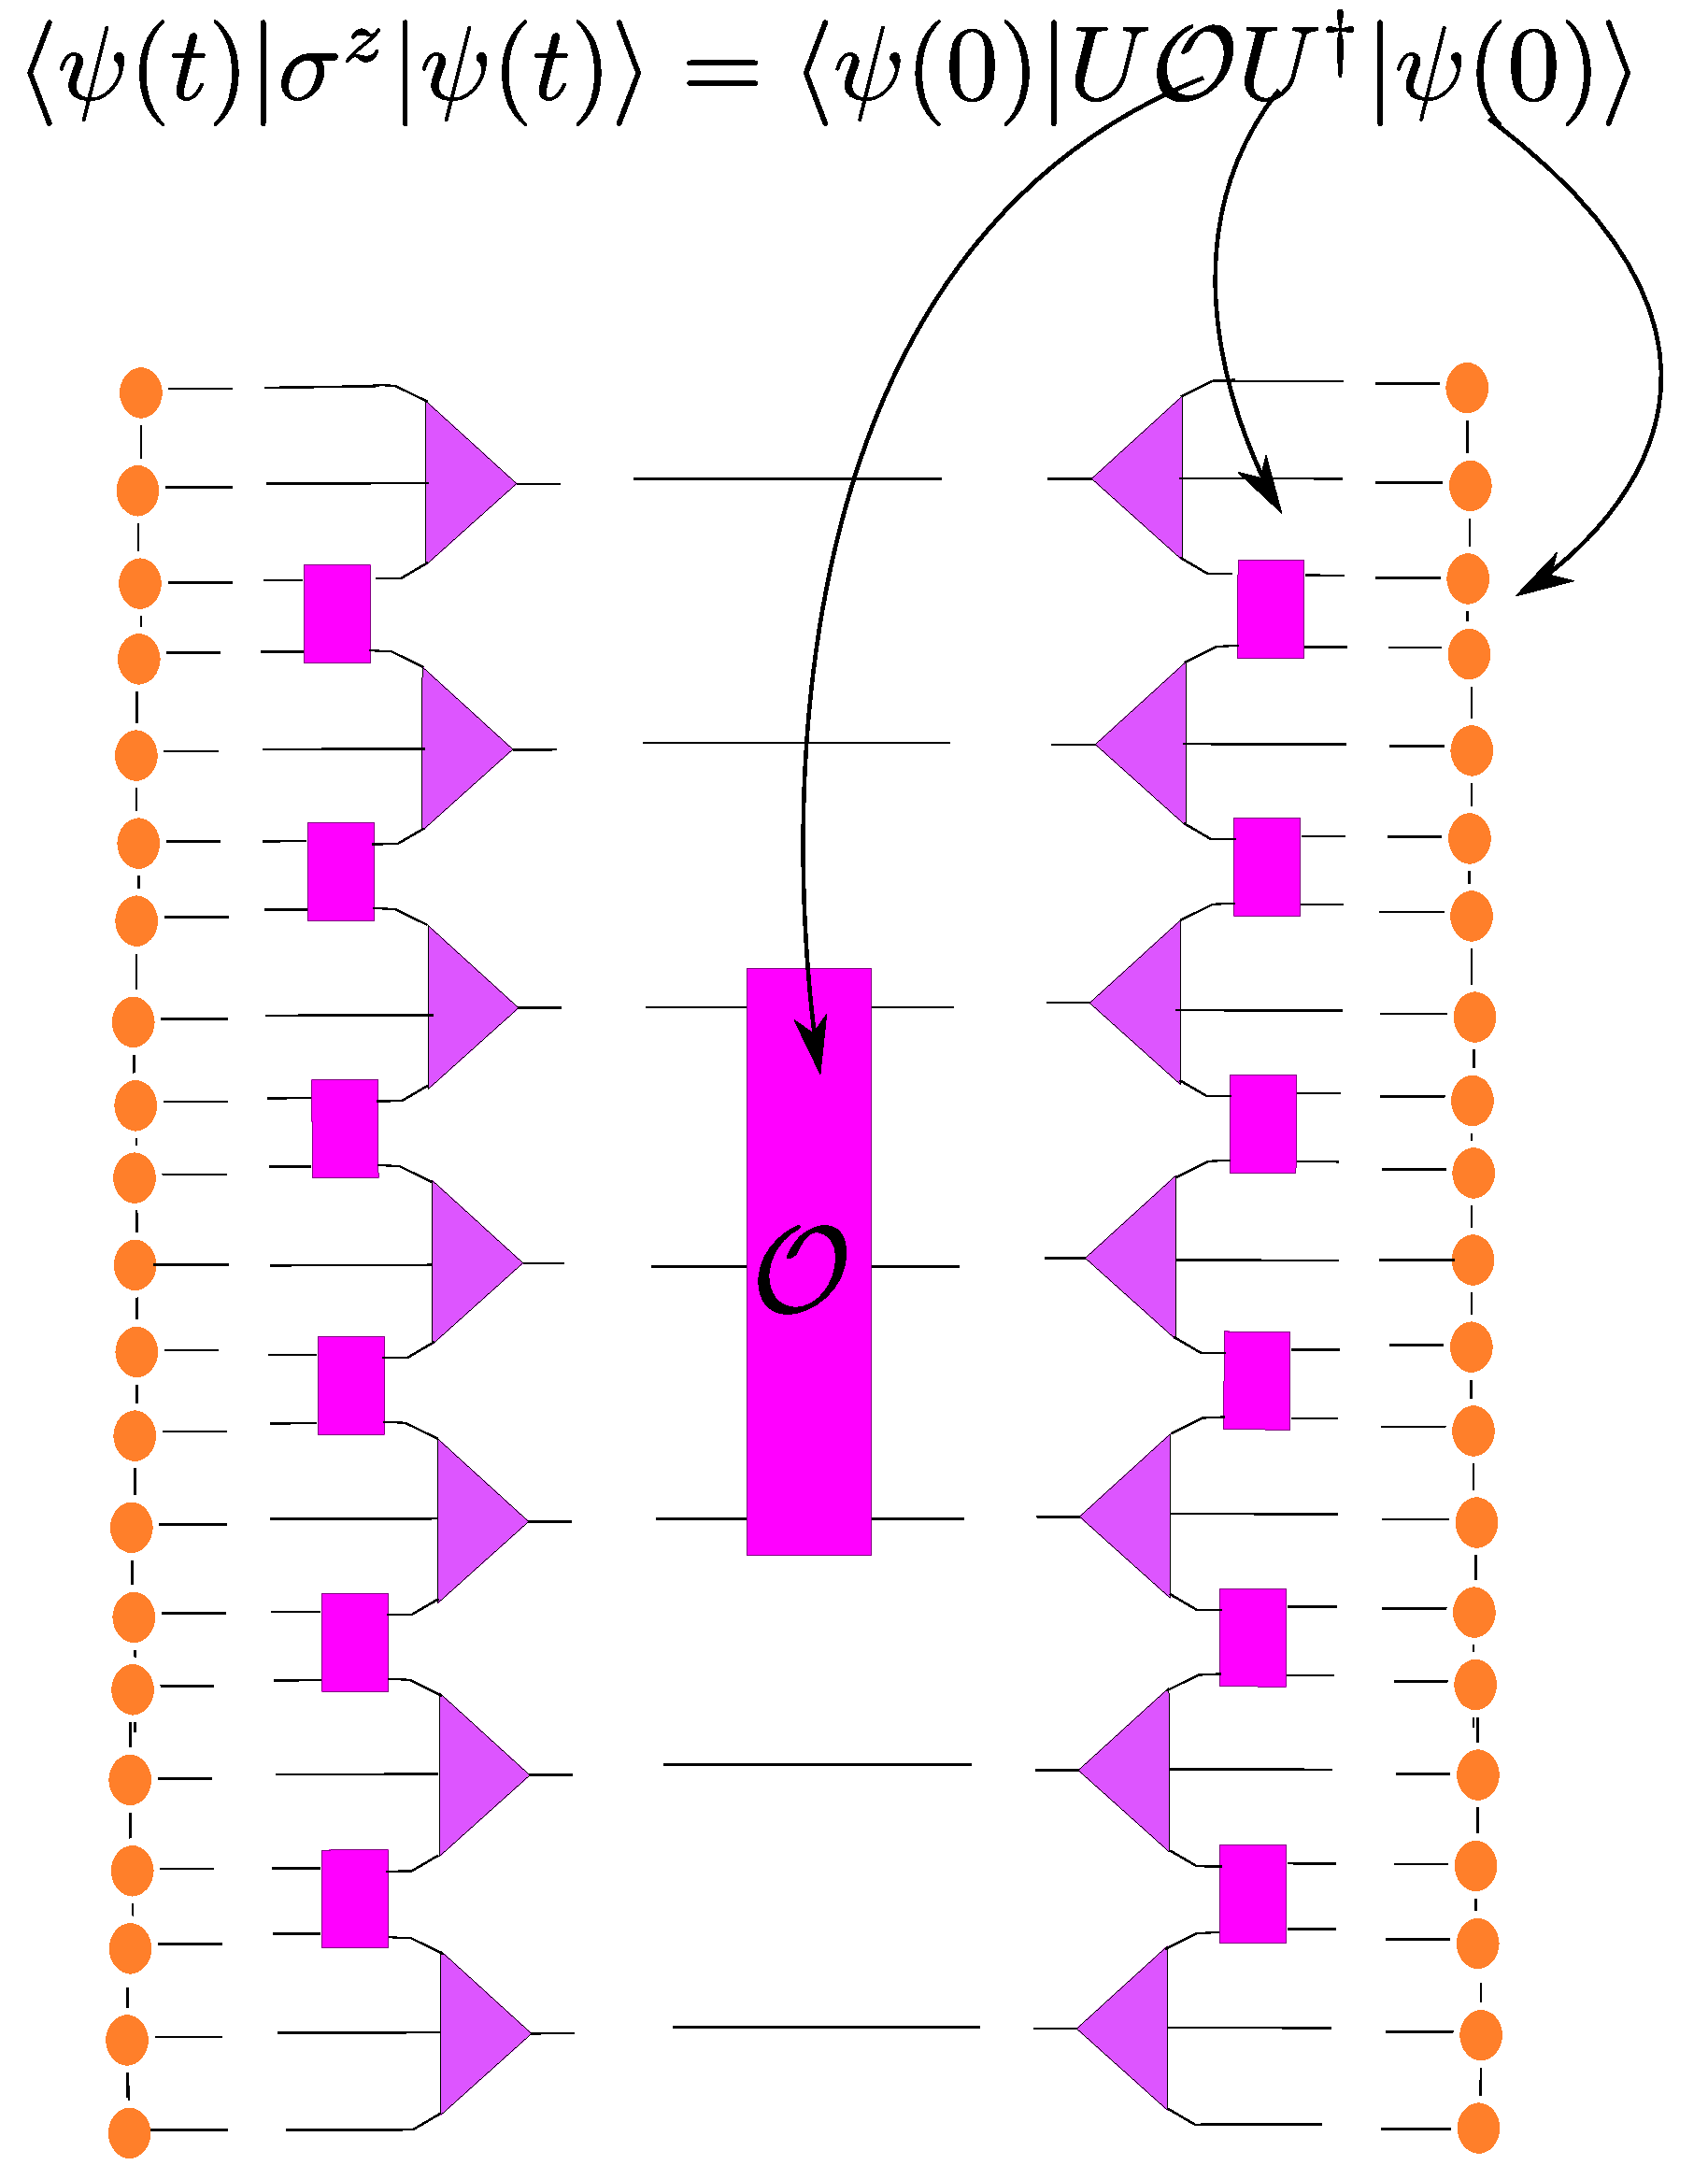
\includegraphics[scale=0.2, angle=0, origin=c]{Final-equation-time}
\end{center}
One could even more simplify the above figure due to cancellation of unitary operators, and come to the final tensor network representation of time evolution,

\begin{center}
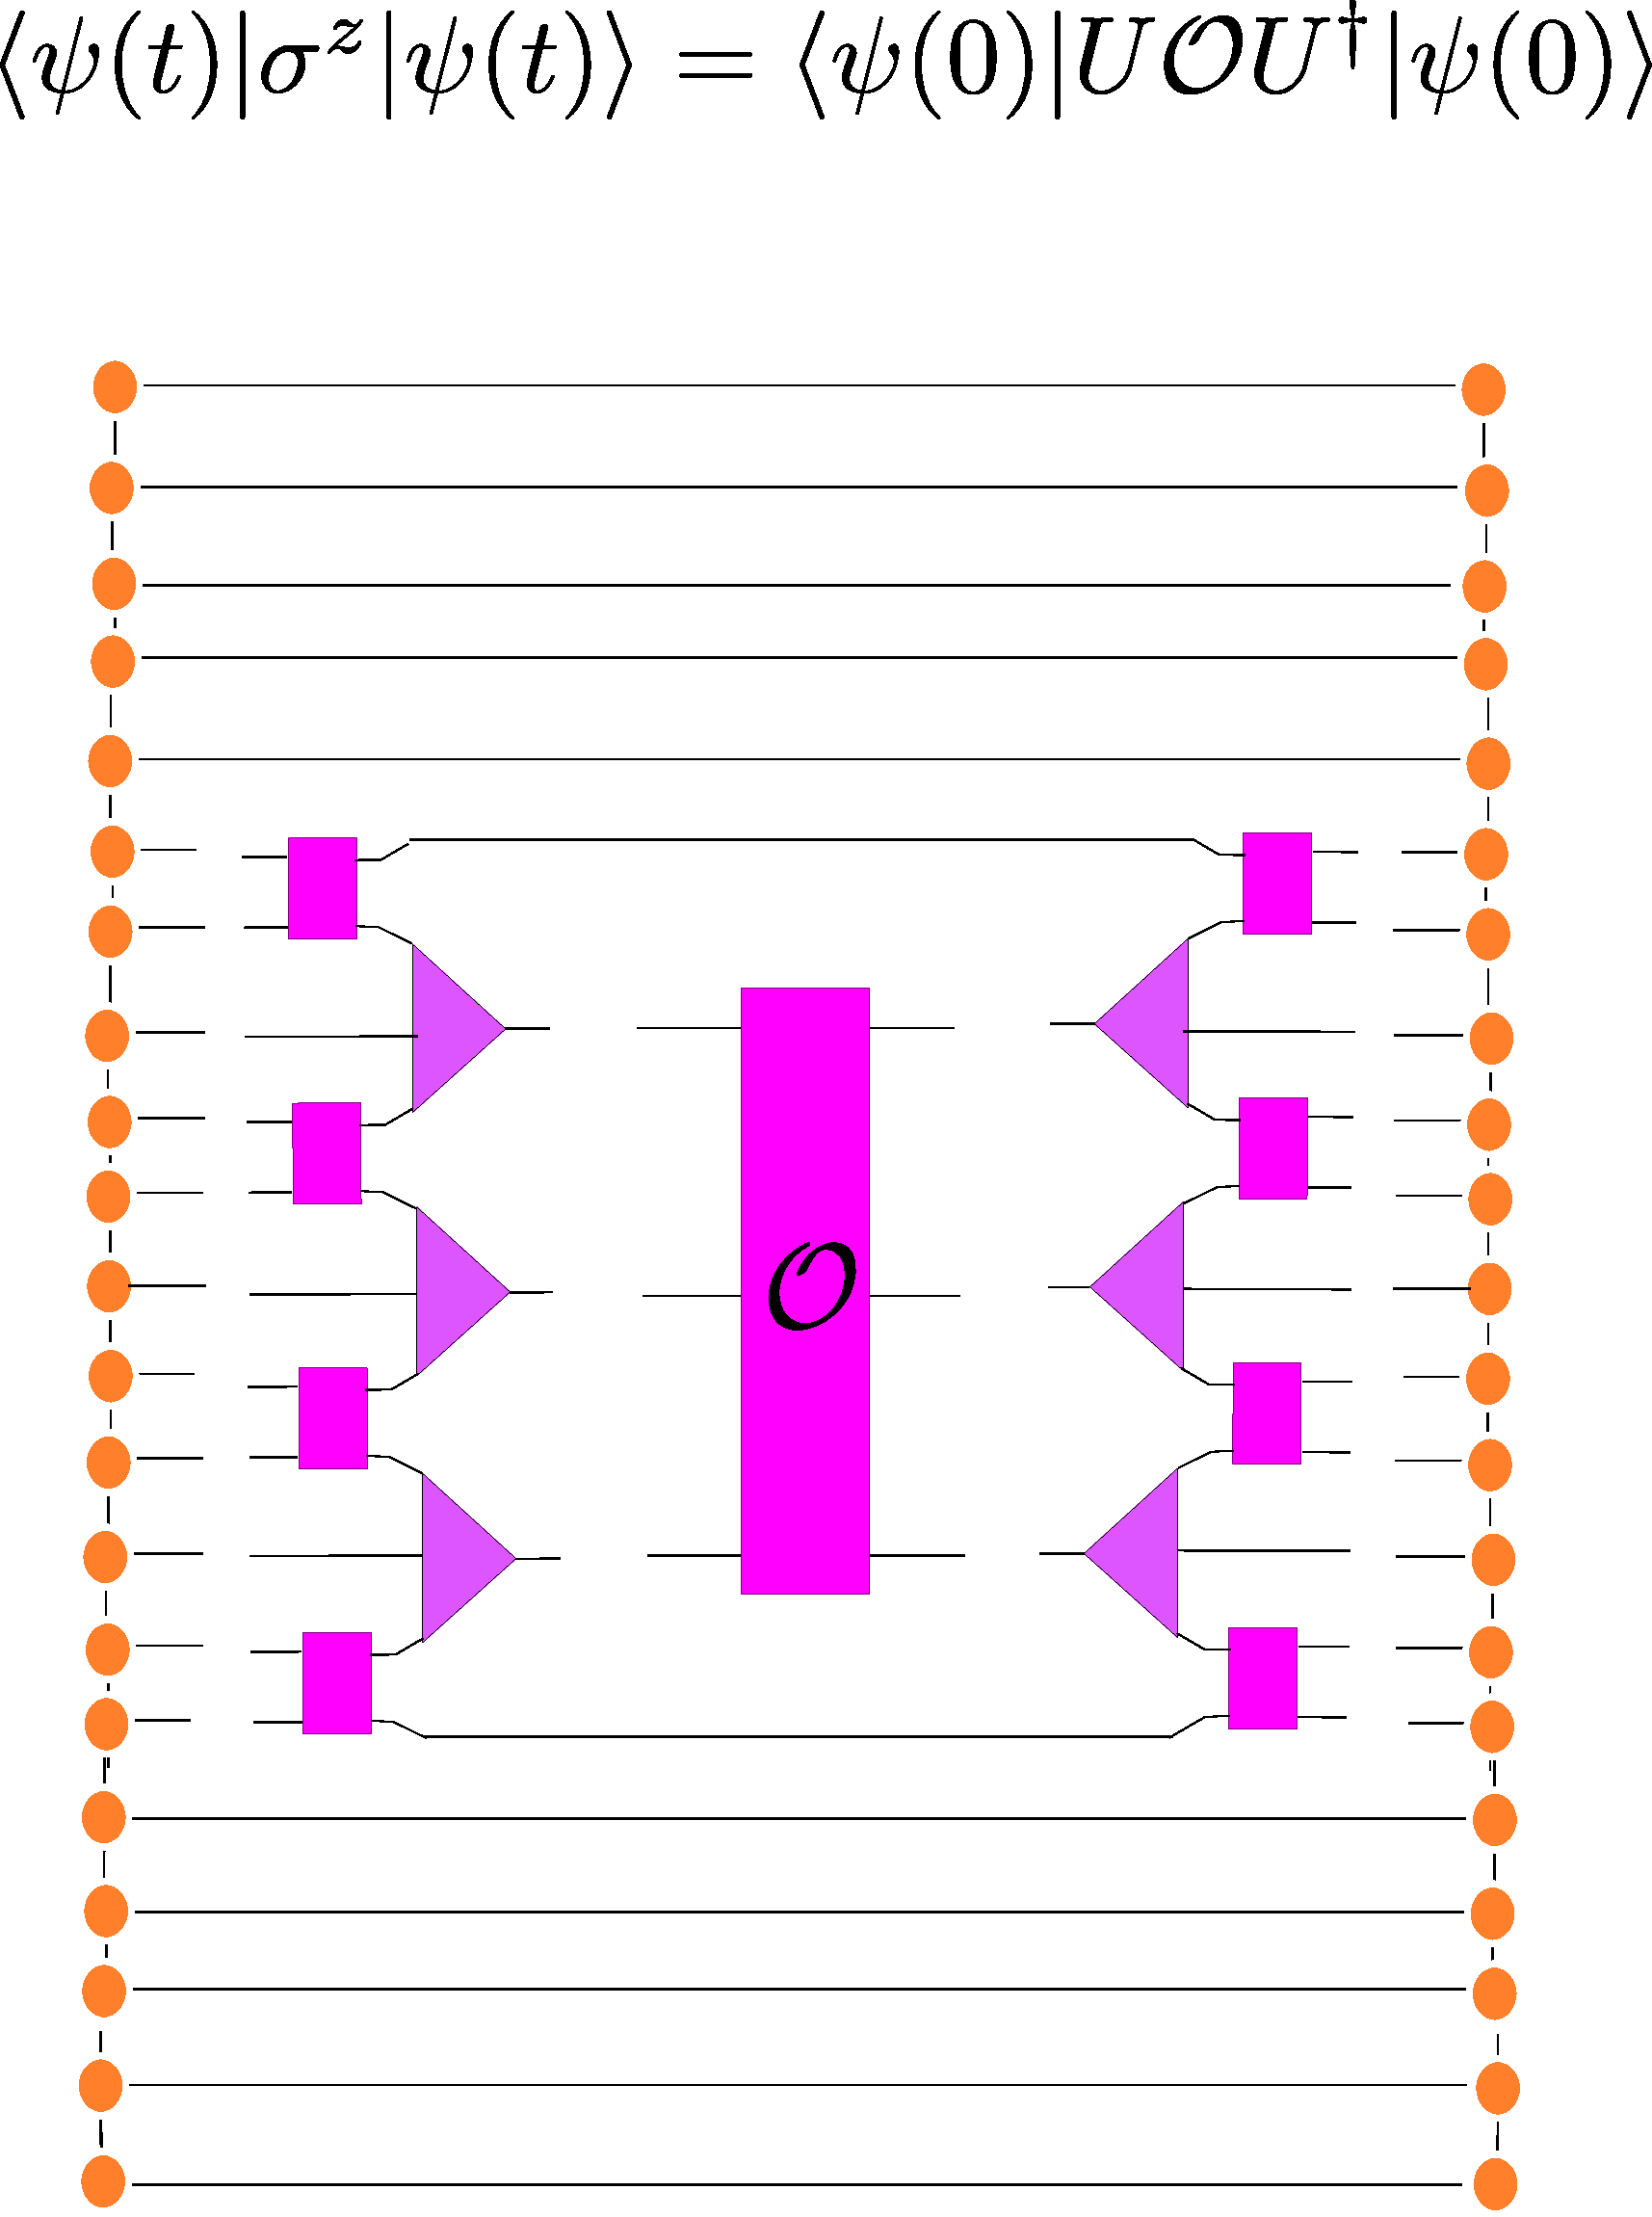
\includegraphics[scale=0.2, angle=0, origin=c]{Finaltimeoperator}
\end{center}
 
One could also consider more layers and obtain similar tensor network representation.  
        
        
\bibliography{references} 
 
\end{document}

